\documentclass[a4paper, 12pt]{article}

\usepackage{amsmath}
\usepackage{amsthm}
\usepackage{amssymb}
\usepackage{enumerate}
\usepackage{hyperref}
\hypersetup{
	colorlinks=true,
	linkcolor=blue,
	filecolor=blue,
	urlcolor=blue,
	citecolor=blue,
}
\usepackage[margin=3cm]{geometry}
\usepackage{mathpazo}
\usepackage{url}
\usepackage{subcaption}
\usepackage{tikz}
\usepackage{pgf}
\usepackage{longtable}
\usepackage{multirow}
\usepackage{graphicx}
\usepackage{pgfplots}
\usepackage{cleveref}
\usepackage{bbm}
\usepackage{wrapfig}
\usepackage{mathrsfs}
\usepackage{afterpage}
\usepackage[svgnames]{xcolor}
\usepackage{minted}
\setminted{tabsize=4}

\numberwithin{equation}{section}
\numberwithin{figure}{section}

\newtheorem{theorem}{Theorem}[section]
\newtheorem{thm}{Theorem}[section]
\newtheorem*{thm*}{Theorem}
\newtheorem*{con*}{Conjecture}
\newtheorem{lem}[thm]{Lemma}
\newtheorem{prop}[thm]{Proposition}
\newtheorem{cor}[thm]{Corollary}
\newtheorem{lemma}[thm]{Lemma}
\newtheorem{conj}[thm]{Conjecture}

\theoremstyle{definition}
\newtheorem{defn}[thm]{Definition}
\newtheorem{remark}[thm]{Remark}
\newtheorem{ex}[thm]{Example}
\newtheorem{quest}[thm]{Question}
\newtheorem{obs}[thm]{Observation}

\renewcommand{\leq}{\leqslant}
\renewcommand{\geq}{\geqslant}
\newcommand{\N}{\mathbb{N}}
\newcommand{\Z}{\mathbb{Z}}
\newcommand{\Q}{\mathbb{Q}}
\newcommand{\R}{\mathbb{R}}
\newcommand{\C}{\mathbb{C}}
\newcommand{\define}[1]{\textit{#1}}

\setcounter{tocdepth}{2}

\allowdisplaybreaks

\title{Software for Mathematical Scientists and Educators}
\author{Joshua Maglione}
\date{\today}

\begin{document}

\maketitle
\tableofcontents

\section*{Introduction}

Communicating mathematics and performing long computations are both vitally
important and challenging. Thankfully there is a wide selection of software to
make these tasks more manageable. In this module, we will explore software used
by everyday mathematicians and scientists. These include biologists, chemists,
computer scientists, data scientists, financial analysts, your friends and
family, educators, engineers, and physicists. 

The goal is to build a foundation by using some of the most ubiquitous software
in the field. This will help students throughout their career in and out of
university. We will cover four topics in this module:
\begin{enumerate} 
	\item Mathematical Typesetting and \LaTeX,
	\item Python and Jupyter Notebooks,
	\item Introduction to Programming,
	\item Symbolic Computation and SageMath.
\end{enumerate}


\section{Mathematical Typesetting and \LaTeX}

With advances in printing and typesetting, the question of how to produce
high-quality mathematical symbols and texts is challenging. Without going
through the history, we now have essentially two main styles of software to
write mathematical formulae, diagrams, and images:
\begin{enumerate}
	\item What-You-See-Is-What-You-Get (WYSIWYG) and
	\item typesetting software (or write-format-preview style).
\end{enumerate}

Software like Microsoft Word, Apple Pages, or LibreOffice Writer are WYSIWYG
editors because you see and edit the document as a final product (regardless of
whether or not it is the final product). This remove the user from having to
remember commands for the document layout, and it has a lower barrier of entry,
which is one of its strongest advantages. However, this is not the norm for
professionals using many mathematical symbols, and the primary disadvantage to
these kinds of software is their sluggish pace---the secondary disadvantage is
that many people struggle to pronounce WYSIWYG causing people to avoid such
software. I certainly cannot pronounce it properly.

One of the first typesetting software for mathematics is \TeX---if not
\textit{the} first. It was written by Donald Knuth\footnote{You can read Knuth's
original memo describing \TeX. He called the memo the ``Preliminary preliminary
description of TEX''~\cite{TeX-draft}.} in 1978~\cite{Knuth-Quanta}, and it is
the cornerstone of the more modern software \LaTeX\ written by Leslie Lamport in
1986~\cite{Lamport}. Although \TeX\ is still used today, \LaTeX\ is far more
popular. The primary disadvantage to these systems is the higher barrier to
entry, but the over-powering advantage is the speed with which one can produce
beautiful and high-quality mathematical symbols. Both \TeX\ and \LaTeX\ are free
and open-source software. 

As alluded to previously, these are typesetting software, so a user writes in a
markup language, usually in a \texttt{tex} file; then the user compiles the
file, and a \texttt{pdf} file is produced. There are other options for output,
but this will be sufficient for us. Another asset is that one can import third
party \LaTeX\ packages to perform more specialized tasks. We will become
familiar with basic \LaTeX\ formatting and use some packages to help construct
beautiful documents. 

For web-based mathematical symbols, MathJax~\cite{MathJax} is primarily used.
However, there is a new, much faster, alternative called KaTeX~\cite{KaTeX}.
Currently, KaTeX can only do a (proper) subset of what MathJax can do, but KaTeX
does enough for everything I have needed for my website---and I have a lot of
complicated formulae on my website. 

\begin{remark}
	Nobody really cares how you pronounce \LaTeX, but some of the popular ways
	are ``law-tech'' and ``lay-tech''. This is because Knuth indicated that
	\TeX\ ought to be pronounced like ``tech'' \cite[Paragraph 2]{TeX-draft}.
	The true non-conformists pronounce it ``lay-techs''. I just prefer to
	pronounce it as \LaTeX.
\end{remark}

\subsection{How to get \LaTeX}

This will not fully cover how to install \LaTeX\ on your own machine, but
hopefully it gives you enough information to help you. It not that \LaTeX\
updates so frequently---in fact \LaTeX\ is still on its second edition
(formatted as \LaTeXe)---it is that packages tend to update or just need
installation. 

For Windows machines, I would recommend MiKTeX. This install LaTeX and comes
with a package manager to help with package installation. A similar version is
available on Mac OS, and it is called MacTeX. Both MiKTeX and MacTeX have
graphical user interfaces. For Linux systems, TeX Live is what I recommend, and
it usually comes pre-installed. It has its own package manager invoked by the
command \texttt{tlmgr}. 

We will primarily use Overleaf in this module. Overleaf is a website that
enables users to interface with \LaTeX\ through cloud-based services. It uses a
``freeium'' model, so that everyone can use the basic features, which will be
sufficient for our module. The major advantage is that one does not have to
worry about installing and package management; all of this is done cloud-side.
Moreover Overleaf simplifies the workflow slightly by allowing for instant
compilation. \#NotSponsored 

\subsection{Workflow and document structure}
\label{sec:workflow}

The basic workflow is perhaps only a little more complicated than how it might
be for WYSIWYG software. Here is the basic workflow. 
\begin{enumerate}
	\item Create a \texttt{tex} file and write \LaTeX\ markup. 
	\item Compile the \texttt{tex} file with the command \texttt{pdflatex}.
	\item Sometimes errors are raised and need to be addressed. It is acceptable
	to cry when this happens; it happens to all of us. If no errors arise, then
	a \texttt{pdf} file is created (or overwritten). 
	\item View and review the output \texttt{pdf} file. 
\end{enumerate}
With the exception of the initial creation of the file, all of these steps are
repeated often. How often? That depends on you and your situation. I would
recommend that, when addressing bugs or typos, that one compile often and review
carefully what has changed. 

The basic format of a \LaTeX\ document is simple. There are three commands that
must be present, and often one tries to adhere to some logical structure due to
collaborations or just to readability over longer periods of time. The first
command that appears in a functioning \texttt{tex} file is the following:
\begin{minted}{latex}
	\documentclass[<options>]{<style>}
\end{minted}
where \texttt{<style>} is replaced with the name of the desired document class
and \texttt{<options>} is replaced with optional parameters for the specific
document class. For example, this current \texttt{pdf} document was built using
\begin{minted}{latex}
	\documentclass[a4paper, 12pt]{article}
\end{minted}
Some other popular document classes, besides \texttt{article}, are 
\begin{itemize}
	\item \texttt{beamer} : for slides,
	\item \texttt{book} : for books,
	\item \texttt{letter} : for letters,
	\item \texttt{standalone} : often used with the package \texttt{TikZ} for
	stand alone pictures.
\end{itemize}
There are also AMS-inspired article and book classes: \texttt{amsart} and
\texttt{amsbook} and KOMA-script versions: \texttt{scrartcl}, \texttt{scrbook},
\texttt{scrlttr2}, and \texttt{scrreprt}. The other two required commands are 
\begin{minted}{latex}
	\begin{document}
	\end{document}
\end{minted}
which encapsulate the main body of the \texttt{tex} file. \Cref{fig:tex-file}
shows the basic layout of a \texttt{tex} file.

\begin{figure}[h]
	\centering
	\begin{tikzpicture}
		\draw (0,-1) rectangle (12,5);
		\draw[fill=Crimson] (0.2, 3.2) rectangle (11.8, 4.3);
		\draw[fill=RoyalBlue] (0.2, -0.3) rectangle (11.8, 2.6);
		\node at (3.8,4.6) {\mintinline{latex}{\documentclass[<options>]{<style>}}};
		\node at (1.85,2.9) {\mintinline{latex}{\begin{document}}};
		\node at (1.65,-0.6) {\mintinline{latex}{\end{document}}};
		\node[White] at (6, 3.75) {\textbf{preamble}};
		\node[White] at (6, 1.15) {\textbf{body}};
	\end{tikzpicture}
	\caption{Basic structure of a \texttt{tex} file.}
	\label{fig:tex-file}
\end{figure}

Although I have never heard anyone refer to the preamble as the head, I think it
makes sense---even if it causes me to stop and use my preamble to figure out
what is meant by it.

\subsection{Source files}

\LaTeX\ \define{source files} are the necessary files needed to compile a
\texttt{tex} file. In particular, a \texttt{tex} file need not be self
contained; there are many reasons why this might be the case. For example, one
might embed graphics in the form of \texttt{jpeg} or \texttt{png} files, or one
might use \textsc{Bib}\TeX\ to dynamically format their bibliography---more on
this in \Cref{sec:bibtex}.

In the process of compiling a \texttt{tex} file to a \texttt{pdf} file, \LaTeX\
produces several auxillary files. These serve specific purposes, but their
particular uses are outside of the scope we will explore. Because so many
additional files are created in the compilation process, it is usually preferred
to build a directory for each \LaTeX\ project. For example, the file names in
the directory for these lecture notes can be seen in \Cref{fig:all-files}.

\begin{figure}[h]
	\centering 
	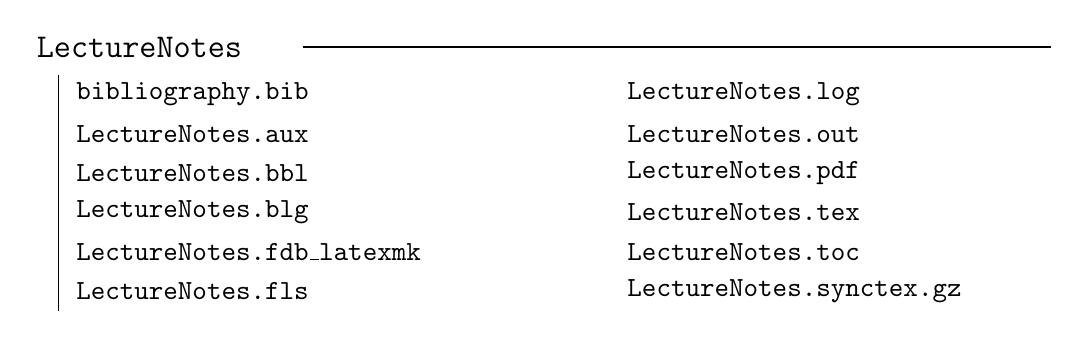
\begin{tikzpicture}
		\node[anchor=west] at (-0.5,3.1) {{\large\texttt{LectureNotes}}};
		\node[anchor=west] at (0,2.5) {\texttt{bibliography.bib}};
		\node[anchor=west] at (0,2) {\texttt{LectureNotes.aux}};
		\node[anchor=west] at (0,1.5) {\texttt{LectureNotes.bbl}};
		\node[anchor=west] at (0,1) {\texttt{LectureNotes.blg}};
		\node[anchor=west] at (0,0.5) {\texttt{LectureNotes.fdb\_latexmk}};
		\node[anchor=west] at (0,0) {\texttt{LectureNotes.fls}};
		\node[anchor=west] at (7,2.5) {\texttt{LectureNotes.log}};
		\node[anchor=west] at (7,2) {\texttt{LectureNotes.out}};
		\node[anchor=west] at (7,1.5) {\texttt{LectureNotes.pdf}};
		\node[anchor=west] at (7,1) {\texttt{LectureNotes.tex}};
		\node[anchor=west] at (7,0.5) {\texttt{LectureNotes.toc}};
		\node[anchor=west] at (7,0) {\texttt{LectureNotes.synctex.gz}};
		\draw (-0.1, 2.75) -- (-0.1, -0.25);
		\draw (3, 3.1) -- (12.5, 3.1);
	\end{tikzpicture}
	\caption{The files in the \texttt{LectureNotes} directory.}
	\label{fig:all-files}
\end{figure}

The only files necessary to compile in \Cref{fig:all-files} are
\texttt{LectureNotes.tex} and \texttt{bibliography.bib}. The rest of the files
are produced by the compilation process. 




\subsection{An introduction to \LaTeX\ syntax}

We will not cover all of the \LaTeX\ syntax here. When we discuss mathematical
symbols and formulae in \Cref{sec:latex-math}, we will cover more. There are
some symbols that \LaTeX\ redefines. For example, \mintinline{latex}{%} 
indicates that the rest of the line should be ignored by the compiler:
\begin{minted}{latex}
	% This is a comment and will be ignored by the
	% LaTeX compiler.
\end{minted}

Commands in \LaTeX\ start with the \mintinline{latex}{\} symbol. We have already
seen examples of this with the following commands:
\begin{minted}{latex}
	\documentclass[a4paper, 12pt]{article}
	\begin{document}
	\end{document}
\end{minted}
Arguments are input using the \mintinline{latex}|{| and \mintinline{latex}|}|
symbols, and multiple arguments would require multiple sets of
\mintinline{latex}|{| and \mintinline{latex}|}|. Optional parameters are input
using the \mintinline{latex}{[} and \mintinline{latex}{]} symbols, but multiple
optional parameters are listed within the single use of \mintinline{latex}{[}
and \mintinline{latex}{]} separated by commas. Not every command requires input
arguments; for example, to format LaTeX as \LaTeX, one uses the command
\mintinline{latex}{\LaTeX}.

One often organizes an article into sections, subsections, subsubsection, etc.
Similarly for books into parts, chapters, sections, etc. These can be easily
managed using standard commands. For example in an \texttt{article} document
class, one can use 
\begin{minted}{latex}
	\section{<title>}
	\subsection{<title>}
	\subsubsection{<title>}
\end{minted}
to produce the desired outcome. For parts and chapters, analogous commands
exist, but errors might be raised if not in a document class that supports them.
For example, \texttt{article} does not support
\mintinline{latex}|\chapter{<title>}|.

Many document classes also have their own way of formatting elements like the
title, author, and date of a document. To access this, usually one includes the
following in their preamble.
\begin{minted}{latex}
	\title{<title>}
	\author{<author>}
	\date{<date>}
\end{minted}
One can type \mintinline{latex}|\date{\today}| to display today's date, provided
the document is compiled today. To display the title, author, and date, include the following command in the body of the document.
\begin{minted}{latex}
	\maketitle
\end{minted}

\subsection{Dynamic bibliographies and \textsc{Bib}\TeX}
\label{sec:bibtex}

Another major advantage to \LaTeX\ is its ability to dynamically format
bibliographies and references. There are a number of different ways to format
bibliographies in \LaTeX, but we will discuss specifically \textsc{Bib}\TeX,
written by Oren Patashnik and Leslie Lamport in the 1980s. 

Have you ever written a document, and after having gotten halfway through, say,
you decide to add another reference?  Depending on the style adopted in your
document, this might have caused you lots of additional work. Not one would you
have to potentially re-order your bibliography, but you might have to change
several references to account for this. Having a dynamically built bibliography
avoids all of this pain. 

To use \textsc{Bib}\TeX, one simply includes two lines wherever the references
should go---usually at the end of the document:
\begin{minted}{latex}
	\bibliography{<bib file name>}
	\bibliographystyle{<style>}
\end{minted}
Thus, in order to use \textsc{Bib}\TeX\ one needs an additional source file: a
\texttt{bib} file. A \texttt{bib} file collects bibliography entries that \textsc{Bib}\TeX\ can read. \Cref{fig:bibtex} provides an example.

\begin{figure}[h]
\begin{minted}{bibtex}
	@book{Macdonald1998,
	    title={Symmetric functions and Hall polynomials},
	    author={Macdonald, Ian Grant},
	    year={1998},
	    publisher={Oxford university press}
	}
\end{minted} 
\caption{A sample \textsc{Bib}\TeX\ entry.}
\label{fig:bibtex}
\end{figure}

In the first line of \Cref{fig:bibtex}, \mintinline{bibtex}{@book} tells
\textsc{Bib}\TeX\ that the bibliography entry is a book. The braces indicate the
block of code designated for this particular entry. And the
\texttt{Macdonald1998} is the \define{tag}---more on this soon. The lines in
between the braces give bibliographical information. As the example illustrates:
we have the book's title, author, year of publication, and publisher. There are
more potential entries one could include as well. The entry will be formatted
relative to the specified style in the output \texttt{pdf} file.

When one wants to cite a particular reference in the body of their \texttt{tex}
file, one simply writes
\begin{minted}{latex}
	\cite[<options>]{<tag>}
\end{minted}
and a citation for that particular entry (relative to the tag) matching the
given style is produced. Using the example in \Cref{fig:bibtex}, we might write
the following sentence in the body of our \texttt{tex} file:
\begin{minted}{latex}
	By \cite[Theorem 3.14]{Macdonald1998}, the proof is complete. 
\end{minted}

The \texttt{bib} file does not need to be ordered. \textsc{Bib}\TeX\ will take
care of ordering all of the bibliography entries properly. Therefore, the
\texttt{bib} file can simply be a dump for bibliography entries. All a user
needs to know are the relevant tags for the references to cite. 

Using \textsc{Bib}\TeX\ modifies the basic workflow described in
\Cref{sec:workflow}. After running \texttt{pdflatex} one needs to run
\texttt{bibtex} twice, and then \texttt{pdflatex} again. Often more crying
ensues. Overleaf and other similar programs can run all of this with one button,
so we will not dwell on this. 

\begin{remark}[Warning]
	\textsc{Bib}\TeX\ can be challenging for newcomers to work with for many
	reasons. Some of the pain is alleviated by Overleaf and other programs, but
	this still does not make it easy.
\end{remark}

\subsection{Mathematical symbols and formulae}
\label{sec:latex-math}

\LaTeX\ provides two primary methods to output mathematical symbols: inline and
as a displayed line. To display maths inline, one initiates with
\mintinline{latex}|$|, ending with the same symbol. One can also start with
\mintinline{latex}|\(| and end with \mintinline{latex}|\)|. Thus,
\mintinline{latex}|$e^x$| is displayed as $e^x$. The Greek alphabet is accessed
by commands like \mintinline{latex}|\pi| for $\pi$ and \mintinline{latex}|\Pi|
for $\Pi$. 

Exponents are indicated by \mintinline{latex}|^| and subscripts by
\mintinline{latex}|_|. Without additional braces, both \mintinline{latex}|^| and
\mintinline{latex}|_| change only the next character. Note the difference in
\mintinline{latex}|$e^{2i\pi}$| as $e^{2i\pi}$ as compared to
\mintinline{latex}|$e^2i\pi$| as $e^2i\pi$. The same holds for subscripts. One
can use both exponents and subscripts; for example
\mintinline{latex}|$M_{ij}^4$| is displayed as $M_{ij}^4$. By using braces one
can nest these operations. For example $x^{x^x}$ is
\mintinline{latex}|$x^{x^x}$| and $x_i^{x_j^2 + x_k^2}$ is
\mintinline{latex}|$x_i^{x_j^2 + x_k^2}$|. 

Note that \LaTeX\ adjusts the height of each line relative to its content. For
this reason and others, some might prefer to display more complicated
expressions in its own displayed line. To accomplish this in \LaTeX\ one uses
\mintinline{latex}|$$| or \mintinline{latex}|\[|, ending with either
\mintinline{latex}|$$| or \mintinline{latex}|\]|, respectively (and not mixing).
For example, 
\begin{minted}{latex}
\[ 
	x_i^{x_j^2 + x_k^2}.
\] 
\end{minted}
produces 
\[ 
	x_i^{x_j^2 + x_k^2}.
\] 

A few more examples of displayed mathematics include the following.
\begin{minted}{latex}
\[ 
	\int_a^b f'(t) dt = f(b) - f(a). 
\] 
\end{minted}
produces 
\[ 
	\int_a^b f'(t) dt = f(b) - f(a). 
\] 
And 
\begin{minted}{latex}
\[
	\lim_{n\to \infty} \sum_{k=1}^n \frac{1}{k} \rightarrow \infty. 
\]
\end{minted}
yields 
\[
	\lim_{n\to \infty} \sum_{k=1}^n \frac{1}{k} \rightarrow \infty. 
\]
Notice that the previous example looks differently when typed inline:\\
\mintinline{latex}|$\lim_{n\to \infty} \sum_{k=1}^n \frac{1}{k} \rightarrow \infty$|\\ 
is displayed as $\lim_{n\to \infty} \sum_{k=1}^n \frac{1}{k}
\rightarrow \infty$, not as elegant I would say. 

\begin{remark}
	There is a heated debate whether or not one should use
	\mintinline{latex}|$$| or the pair \mintinline{latex}|\[| and
	\mintinline{latex}|\]|. It is very controversial, and by now you see where I
	stand. (This is of course a joke---perhaps some people are loyal to a
	particular style, but it is completely pointless. Bring on the haters.)
\end{remark}

\subsection{\LaTeX\ Environments}
\label{sec:latex-envs}

One of the general blueprints of \LaTeX\ markup is an \define{environment}. A
\LaTeX\ environment has the following basic structure:
\begin{minted}{latex}
	\begin{<environment>}     % Explicit start of environment
		%
		% Content
		%
	\end{<environment>}       % Explicit end of environment
\end{minted}
One could say that a \texttt{tex} file is essentially a \LaTeX\ environment
using \texttt{document}, but people do not say that. That would be ridiculous;
let's not promote that. 

\subsubsection{The \texttt{equation} environment}

The displayed lines of math from \Cref{sec:latex-math} can be viewed as an
environment. One can even do this in an environment format. For example,
\begin{minted}{latex}
	\begin{equation}
		\sum_{n=1}^\infty \frac{1}{n^s} 
			= \prod_{p \text{ prime}} \frac{1}{1 - p^{-s}} 
	\end{equation}
\end{minted}
yields
\begin{equation}
	\sum_{n=1}^\infty \frac{1}{n^s} 
		= \prod_{p \text{ prime}} \frac{1}{1 - p^{-s}} 
\end{equation}

\begin{remark}\label{rem:labels}
	As a digression, notice in the previous example that there is a reference
	number to the right of the equation, namely (1.1). If we provide a label for
	the equation, we can reference that label anywhere in the document and it
	will produce the correct reference number. For example 
	\begin{minted}{latex}
		\begin{equation}\label{eqn:Euler-decomp}
			\sum_{n=1}^\infty \frac{1}{n^s} 
				= \prod_{p \text{ prime}} \frac{1}{1 - p^{-s}} 
		\end{equation}
	\end{minted}
	yields 
	\begin{equation}\label{eqn:Euler-decomp}
		\sum_{n=1}^\infty \frac{1}{n^s} 
			= \prod_{p \text{ prime}} \frac{1}{1 - p^{-s}} 
	\end{equation}
	and we can reference it with \mintinline{latex}|\ref{eqn:Euler-decomp}|
	producing \ref{eqn:Euler-decomp}. Equations usually have special
	formatting---note the parentheses---so to account for this, there is a
	special way to reference equations:
	\mintinline{latex}|\eqref{eqn:Euler-decomp}| yields
	\eqref{eqn:Euler-decomp}.
\end{remark}

\subsubsection{The \texttt{align} environment}

Another mathematical environment is \texttt{align}. \textit{This uses a very
common package that should be used every time. More about this in
\Cref{sec:latex-packages}}.
\begin{minted}{latex}
	\begin{align} 
		\sum_{n=1}^{\infty} \frac{1}{n^2} 
		&= 1 + \frac{1}{4} + \frac{1}{9} + \cdots \\
		&= \frac{\pi^2}{6} . 
	\end{align}
\end{minted}
yields 
\begin{align} 
	\sum_{n=1}^{\infty} \frac{1}{n^2} 
	&= 1 + \frac{1}{4} + \frac{1}{9} + \cdots \\
	&= \frac{\pi^2}{6} . 
\end{align}

A few aspects to note. First observe that each line has a reference number; see
\Cref{rem:labels} for a brief explanation on how to take advantage of these
reference numbers. (To actually reference that particular remark, I am using
label and ref commands. When does the rabbit hole end?!) The standard way to
turn off these reference numbers, for example if they are unused or unwanted, is
to append the environment name with \texttt{*}. Thus, \texttt{equation*} and
\texttt{align*} will not produce reference numbers on the side. 

\subsubsection{The \texttt{center} environment}

The \texttt{center} environment center justifies the text within the
environment. For example 
\begin{minted}{latex}
	\begin{center}
		This text is centered.
	\end{center}
\end{minted}
produces
\begin{center}
	This text is centered.
\end{center}

\subsubsection{the \texttt{tabular} environment}

The \texttt{tabular} environment is used for creating tables in \LaTeX. It
allows one to specify the alignment, formatting, and content of each cell within
the table. For example, we can create a center-justified table with the following code:
\begin{minted}{latex}
	\begin{center}
	\begin{tabular}{|l|c|r|}
		\hline
		\textbf{My} & \textbf{Favorite} & \textbf{Table} \\
		\hline
		Look, & Ma & no \\
		\hline
		hands! & he & shouted \\
		\hline 
		before & crashing & (more data) \\
		\hline
	\end{tabular}
	\end{center}
\end{minted}
It produces the following table:
\begin{center}
	\begin{tabular}{|l|c|r|}
		\hline
		\textbf{My} & \textbf{Favorite} & \textbf{Table} \\
		\hline
		Look, & Ma & no \\
		\hline
		hands! & he & shouted \\
		\hline 
		before & crashing & (more data) \\
		\hline
	\end{tabular}
\end{center}
The argument \mintinline{latex}{{|l|c|r|}} indicates that the table should have
four vertical lines; the cells in the first column should be left-justified; the
cells in the second column should be center-justified; and the cells in the
third column should be right-justified. The \mintinline{latex}|\hline| command
is used to draw horizontal lines between rows. The symbol \mintinline{latex}|&|
is used to separate cells within a given row, and the symbol
\mintinline{latex}|\\| is used to create new rows in the table. 

\subsubsection{The \texttt{enumerate} and \texttt{itemize} packages}

The \texttt{enumerate} environment is employed to create ordered lists. It
enables the user to specify items within the list, automatically numbering them
in the desired format---it's magical moment when you do not have to renumber
items in your list. The following 
\begin{minted}{latex}
	\begin{enumerate}
		\item First item,
		\item Second item,
		\item Another item,
		\item I am losing count,
		\item but it does not matter because I do not,
		\item have to,
		\item count!
	\end{enumerate}
\end{minted}
produces the following numbered list:
\begin{enumerate}
	\item First item,
	\item Second item,
	\item Another item,
	\item I am losing count,
	\item but it does not matter because I do not,
	\item have to,
	\item count!
\end{enumerate}
Notices the \mintinline{latex}|\item| command is used to delineate individual
entries within the list. An \texttt{enumerate} without an
\mintinline{latex}|\item| is like a goose around her goslings---easily angered,
it's best to steer clear from them, trust me.

One can skip or simply change the numbering using
\mintinline{latex}|\setcounter|, but I will not go into the details here. There
are plenty of examples on the Internet. 

You can nest enumerate. For example:
\begin{minted}{latex}
	\begin{enumerate}
		\item Look at me.
		\item \begin{enumerate}
			\item I can make
			\item nested enumerates.
		\end{enumerate}
		\item So cool.
	\end{enumerate}
\end{minted}
produces 
\begin{enumerate}
	\item Look at me.
	\item \begin{enumerate}
		\item I can make
		\item nested enumerates.
	\end{enumerate}
	\item So cool.
\end{enumerate}

The \texttt{itemize} environment works in much the same way as
\texttt{enumerate} except that produces unordered lists. The default is bullet
points. 

\subsection{Some \LaTeX\ packages}
\label{sec:latex-packages}

\LaTeX\ packages are essential tools that enhance the functionality of \LaTeX.
Packages are sets of additional commands and features that extend the
capabilities of the basic \LaTeX\ system, often for specialized tasks. Packages
are, therefore, designed to address specific needs, making \LaTeX\ highly
versatile and adaptable to various document requirements.

To use a \LaTeX\ package, you need to include it in the preamble of your
document. Recall from \Cref{sec:workflow} that the preamble is the part of the
document after \mintinline{latex}|\documentclass[<options>]{<style>}| and before
\mintinline{latex}|\begin{document}|. To include a package, one first needs it
to be installed in the local machine---or one can use Overleaf and avoid
thinking about this. Then in the document (often just after the
\mintinline{latex}|\documentclass[<options>]{<style>}|), one writes 
\begin{minted}{latex}
	\usepackage[<options>]{<package name>}
\end{minted}
Sometimes the \texttt{<options>} are relevant, and sometimes they are not. For
example, the first few lines of this document look like 
\begin{minted}{latex}
	\documentclass[a4paper, 12pt]{article}
	\usepackage{amsmath}
	\usepackage{amsthm}
	\usepackage{amssymb}
	\usepackage{enumerate}
	\usepackage{hyperref}
	\usepackage[margin=3cm]{geometry}
\end{minted}

We will mention a few packages that might be particularly relevant. We will give
brief summaries of their capabilities, but those interested should check the
documentation---or probably more realistically, type exactly what you are
looking for in Google and go from there.

\subsubsection{The \texttt{amsmath} package}
\label{sec:amsmath}

One of the most useful packages for mathematical output is
\texttt{amsmath}~\cite{amsmath}. It provides numerous environments and commands
for formatting equations, aligning mathematical expressions, and handling
mathematical symbols. One of the environments provided was discussed in
\Cref{sec:latex-envs}: \texttt{align}. 

The \texttt{amsmath} package provides environments for matrices:
\texttt{matrix}, \texttt{bmatrix}, \texttt{pmatrix}. The following code 
\begin{minted}{latex}
	\[
		\begin{pmatrix}
			1 & 2 \\
			3 & 4 \\
		\end{pmatrix}
	\]
\end{minted}
produces 
\[
    \begin{pmatrix}
        1 & 2 \\
        3 & 4 \\
    \end{pmatrix}
\]
One separates elements in a given row using the \mintinline{latex}|&|, and one
uses \mintinline{latex}|\\| to start a new row. It additionally offers commands
\mintinline{latex}|\dfrac| and \mintinline{latex}|\tfrac|, which are like
\mintinline{latex}|\frac|, the former is in display style and the latter in
inline style.


\subsubsection{The \texttt{amsthm} package}

The \texttt{amsthm} package is specifically designed to facilitate the
typesetting of theorems, lemmas, definitions, and similar structures in a
document. It is part of the collection of \LaTeX\ packages offered by the
American Mathematical Society (along with \texttt{amsmath}), offering enhanced
customization and consistency in the presentation of mathematical theorems and
related structures.

The key features of the package are 
\begin{enumerate}
	\item Theorem-like Environments: Allows you to define new theorem-like
	structures (like Theorem, Lemma, Corollary, Proposition, Definition,
	Example, Remark).
	\item Customization: Provides options to customize the style of theorem-like
	environments, such as italicized or normal text, numbering, and shared or
	independent counters.
	\item Proof Environment: Offers a dedicated proof environment for
	typesetting proofs, automatically adding a QED symbol at the end.
\end{enumerate}

One needs to first define the theorem-like environment. There are two main commands for doing this:
\begin{minted}{latex}
	\newtheorem{<name>}{<printed output>}[<numbered within>]
	\newtheorem{<name>}[<numbered like>]{<printed output>}
\end{minted}
As an example, we define the following in our preamble.
\begin{minted}{latex}
	\newtheorem{theorem}{Theorem}[section]
\end{minted}
Now we can write theorems in a dedicated environment using 
\begin{minted}{latex}
	\begin{theorem}
		The equation $x^n + y^n = z^n$ has no solution in 
		the positive integers for $n \geq 3$.
	\end{theorem}
\end{minted}
This yields the following.

\begin{theorem}
	The equation $x^n + y^n = z^n$ has no solution in 
	the positive integers for $n \geq 3$.
\end{theorem}

We can cross-reference by using \mintinline{latex}|\label{<tag>}| and
\mintinline{latex}|\ref{<tag>}|. Let's label our theorem:
\begin{minted}{latex}
	\begin{theorem}\label{Fermat}
		The equation $x^n + y^n = z^n$ has no solution in 
		the positive integers for $n \geq 3$.
	\end{theorem}
\end{minted}
This produces
\begin{theorem}\label{Fermat}
	The equation $x^n + y^n = z^n$ has no solution in 
	the positive integers for $n \geq 3$.
\end{theorem}
\noindent We can reference Theorem~\ref{Fermat} by \mintinline{latex}|\ref{Fermat}|.

\subsubsection{The \texttt{graphicx} package} 

The \texttt{graphicx} \cite{graphicx} package is a powerful tool for including
and manipulating graphics (or images) within documents. It extends the basic
capabilities of \LaTeX\ by providing commands for inserting images, scaling,
rotating, and controlling their placement. For example 
\begin{minted}{latex}
	\begin{center}
		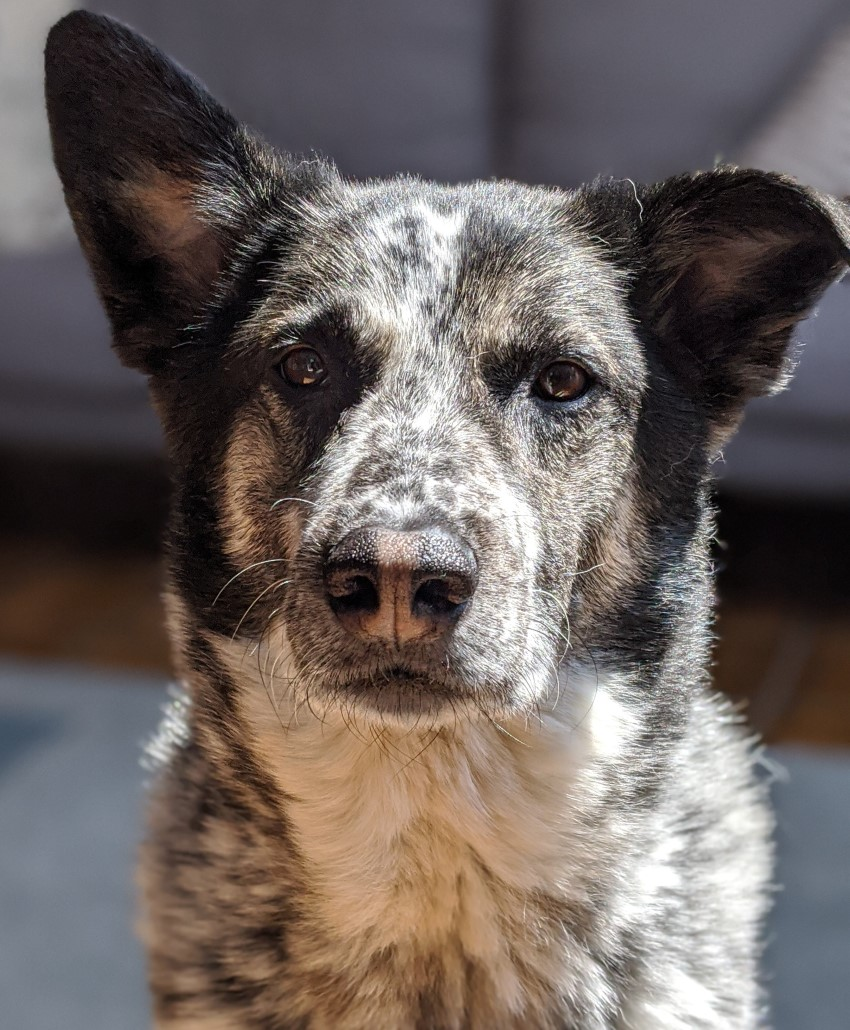
\includegraphics[scale=0.2]{imgs/Sherlock.jpg}
	\end{center}
\end{minted}
produces a picture of my dog
\begin{center}
	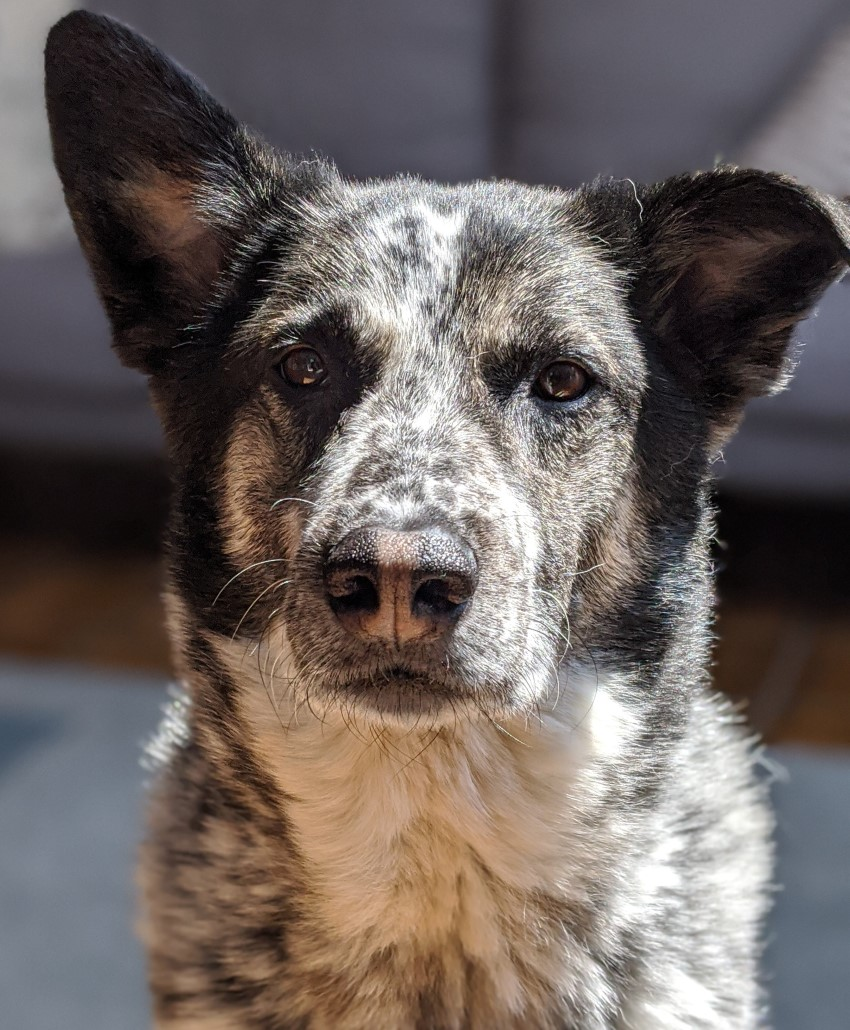
\includegraphics[scale=0.2]{imgs/Sherlock.jpg}
\end{center}


\subsubsection{What now?}

There are over 4000 packages, so I guess we should go through them all one by
one. This will surely be on the exam. I recommend, in particular,  checking out
the following packages---at least see how people might use these packages. 
\begin{itemize}
	\item \texttt{hyperref} : Enables references and citations to produce hyperlinks within the \texttt{pdf} file. (This file uses it.)
	\item \texttt{listings} : Displays code and pseudo-code in a structure block.
	\item \texttt{siunitx} : For those working often with SI units, this can help manage it all.
	\item \texttt{tikz} : Very powerful image producing package. The possibilities are stunning.
\end{itemize}




\newpage

\bibliography{bibliography}
\bibliographystyle{plain}

\end{document}